%! Author = matt_dumont
%! Date = 4/12/23

%----------------------------------------------------------------------------------------
% set document class
\documentclass[11pt]{article}
%----------------------------------------------------------------------------------------

%%%%%%%%%%%%%%%%%%%%%%%%%%%%-----------------------------------%%%%%%%%%%%%%%%%%%%%%%%%%%%
%	REPORT INFORMATION
%----------------------------------------------------------------------------------------

\newcommand{\reporttitle}{The Power of the Current Monitoring Network to Detect Nitrate Reductions in the Selwyn Waihora Zone}

\newcommand{\projcode}{Z22014OLW}
\newcommand{\nthreport}{4}
\newcommand{\projectname}{Selwyn Waihora Detection Power}


\newcommand\authors{
    \textbf{Matt Dumont:} \textit{Lead Computational Hydrogeologist, Kōmanawa Solutions Ltd}\\\\
    \textbf{Zeb Etheridge:} \textit{Director \& Principal Water Resource Scientist, Kōmanawa Solutions Ltd}\\\\
}

\newcommand\authorcite{Dumont and Etheridge}

\newcommand\client{Environment Canterbury}
\newcommand\reportstartdate{01/09/2023}
\newcommand\reportenddate{\today}

% DRAFT WATERMARK %todo RM THIS FOR FINAL
\usepackage{draftwatermark}
\SetWatermarkScale{5}
\SetWatermarkLightness{0.9}

%%%%%%%%%%%%%%%%%%%%%%%%%%%%-----------------------------------%%%%%%%%%%%%%%%%%%%%%%%%%%%
%	DOCUMENT PREAMBLE / SETUP
%----------------------------------------------------------------------------------------
% Packages
%----------------------------------------------------------------------------------------
\usepackage[sfdefault]{carlito} % Use the Carlito font
\graphicspath{{figures/}{./}{ksl_fig/}} % Specifies where to look for included images (trailing slash required)
\usepackage[table]{xcolor}
\usepackage{array}
\usepackage{xstring}
\usepackage{lipsum}
\usepackage[utf8]{inputenc}
\usepackage[T1]{fontenc}
\usepackage[title,titletoc,toc]{appendix} % Required for the appendices section
\usepackage{titletoc} % Required for manipulating the table of contents
\usepackage{booktabs} % Required for nicer horizontal rules in tables
\usepackage{amssymb} % Required for some math elements
\usepackage{mathtools} % Required for some math elements
\usepackage[ddmmyyyy]{datetime} % Sets date format to yyyy-mm-dd
\usepackage{geometry} % Required for adjusting page dimensions and margins
\usepackage{titlesec} % Required for manipulating the section titles
\usepackage[skins, most, many, listings]{tcolorbox} % create breakaway boxes
\usepackage[backref]{hyperref} % Required for adding links and customizing them
\usepackage{enumitem, datatool} % Required for sorted list % Required for list customization
\usepackage[labelfont=bf]{caption}
\usepackage{fancyhdr} % Required for custom headers and footers
\usepackage{scrextend} % Required for indenting paragraphs
\usepackage{glossaries-extra}
\usepackage{etoolbox}
\usepackage{ksl_fig/kslfigure}
\usepackage{natbib}
\usepackage{pdflscape}
\usepackage{truncate}
\usepackage{dirtytalk}

%----------------------------------------------------------------------------------------
% GLOSSARY SETUP
%----------------------------------------------------------------------------------------
\makeglossaries  %keynote if glossery isn't made then check run configurations and ensure makeglosseries is enabled as an extension
\setabbreviationstyle[acronym]{short-long}
\GlsXtrEnableEntryCounting
{acronym}% list of categories to use entry counting
{3}% trigger value (only add to glossary if count > 3)
%! Author = matt_dumont
%! Date = 4/12/23

% todo replace with general_acronym_list.tex...

\newacronym{no3n}{NO\textsubscript{3}-N}{nitrate nitrogen}
\newacronym{olw}{OLW}{Our Land and Water National Science Challenge}
\newacronym{mav}{MAV}{maximum acceptable value}
\newacronym{natbotno3}{NBL-NO\textsubscript{3}-N}{National Bottom Line for Nitrate Nitrogen}
\newacronym{ecan}{ECAN}{Environment Canterbury}
\newacronym{mfe}{MfE}{Ministry for the Environment}
\newacronym{moh}{MoH}{Ministry of Health}
\newacronym{pc1}{PC\textsubscript{1}}{Plan Change 1}
\newacronym{proj_repo}{Project Github Repo.} {Project Github Repository (https://github.com/Komanawa-Solutions-Ltd/Z22014OLW\_SelwynCaseStudy)}

\newacronym{epfm}{EPFM}{exponential piston flow model}
\newacronym{mrt}{MRT}{mean residence time}

%-----------------------------------------------------------------------------------------
% CUSTOM COLORS
%-----------------------------------------------------------------------------------------
\definecolor{ksldarkblue}{RGB}{49,83,125}
\definecolor{ksllightblue}{RGB}{64,163,219}
\definecolor{kslvlblue}{RGB}{215,236,247}
%----------------------------------------------------------------------------------------
% HYPERLINK SETUP
%----------------------------------------------------------------------------------------
\hypersetup{
    colorlinks,
    linkcolor={ksldarkblue},
    citecolor={red!80!black},
    urlcolor={blue!80!black}
}

%----------------------------------------------------------------------------------------
% define breakaway box
\newtcolorbox[auto counter,number within=section,list inside=bab]{breakawaybox}[2][]{
    enhanced,colframe=ksldarkblue,colback=kslvlblue,fonttitle=\bfseries,
    colbacktitle=ksllightblue, coltitle=black,center title,
    title=Box~\thetcbcounter: #2,#1}

\makeatletter
\newcommand\tcb@cnt@breakawayboxautorefname{Box}
\makeatother


%----------------------------------------------------------------------------------------
%	MARGINS and SPACING
%----------------------------------------------------------------------------------------
\setlength{\parindent}{0pt} % Paragraph indentation
\setlength{\parskip}{10pt} % Vertical space between paragraphs
\setcounter{tocdepth}{2} % Show entries in the table of contents down to subsections
\geometry{
    a4paper,
    total={170mm,257mm},
    left=20mm,
    top=20mm,
}
%----------------------------------------------------------------------------------------
% heading enumeration and spacing etc.
%----------------------------------------------------------------------------------------
\setcounter{secnumdepth}{4} % Number headings down to subparagraphs (level 5),
\setcounter{tocdepth}{4} % Show headings down to subparagraphs (level 5) in the table of contents

% set all section headings to ksl dark blue
\titleformat{\section}
{\normalfont\Large\bfseries\color{ksldarkblue}}{\thesection}{1em}{}

\titleformat{\subsection}
{\normalfont\large\bfseries\color{ksldarkblue}}{\thesubsection}{1em}{}

\titleformat{\subsubsection}
{\normalfont\normalsize\bfseries\color{ksldarkblue}}{\thesubsubsection}{1em}{}

\titleformat{\paragraph}
{\normalfont\normalsize\bfseries\color{ksldarkblue}}{\theparagraph}{1em}{}
\titlespacing*{\paragraph}{\parindent}{3.25ex plus 1ex minus .2ex}{.75ex plus .1ex}

\titleformat{\subparagraph}
{\normalfont\normalsize\bfseries\slshape\color{ksldarkblue}}{\thesubparagraph}{1em}{}
\titlespacing*{\subparagraph}{\parindent}{3.25ex plus 1ex minus .2ex}{.75ex plus .1ex}

%----------------------------------------------------------------------------------------
% Table formatting
%----------------------------------------------------------------------------------------
\NewTblrTheme{fancy_tab}{
    \SetTblrStyle{caption-tag}{font=\bfseries}
}
\NewTblrEnviron{ksltable}
\SetTblrOuter[ksltable]{}
\SetTblrInner[ksltable]{
    rowhead = 1,
    hlines, %horizontal lines
    row{odd} = {kslvlblue}, % alternate row colors
    row{even} = {white}, % alternate row colors
    row{1} = {font=\bfseries, ksldarkblue, fg=white}, % header row
}

\NewTblrEnviron{ksltablelong}
\SetTblrOuter[ksltablelong]{long, theme=fancy_tab}
\SetTblrInner[ksltablelong]{
    rowhead = 1,
    hlines, %horizontal lines
    vlines,
    row{odd} = {kslvlblue}, % alternate row colors
    row{even} = {white}, % alternate row colors
    row{1} = {font=\bfseries, ksldarkblue, fg=white} % header row
}

%----------------------------------------------------------------------------------------
% Figure, table, equation numbering scheme
%----------------------------------------------------------------------------------------
\numberwithin{equation}{section} % Number equations within sections (i.e. 1.1, 1.2, 2.1, 2.2 instead of 1, 2, 3, 4)
\numberwithin{figure}{section} % Number figures within sections (i.e. 1.1, 1.2, 2.1, 2.2 instead of 1, 2, 3, 4)
\numberwithin{table}{section} % Number tables within sections (i.e. 1.1, 1.2, 2.1, 2.2 instead of 1, 2, 3, 4)

%----------------------------------------------------------------------------------------
% set section/appendix autoref names
%----------------------------------------------------------------------------------------
\def\sectionautorefname{Section}
\def\subsectionautorefname{Section}
\def\subsubsectionautorefname{Section}
\def\paragraphautorefname{Section}
\def\subparagraphautorefname{Section}
\def\appendixautorefname{Appendix}

%----------------------------------------------------------------------------------------
% appendix autoref patch from https://tex.stackexchange.com/questions/149807/autoref-subsections-in-appendix
%----------------------------------------------------------------------------------------

\makeatletter
\patchcmd{\hyper@makecurrent}{%
    \ifx\Hy@param\Hy@chapterstring
    \let\Hy@param\Hy@chapapp
    \fi
}{%
    \iftoggle{inappendix}{%true-branch
    % list the names of all sectioning counters here
        \@checkappendixparam{chapter}%
        \@checkappendixparam{section}%
        \@checkappendixparam{subsection}%
        \@checkappendixparam{subsubsection}%
        \@checkappendixparam{paragraph}%
        \@checkappendixparam{subparagraph}%
    }{}%
}{}{\errmessage{failed to patch}}

\newcommand*{\@checkappendixparam}[1]{%
    \def\@checkappendixparamtmp{#1}%
    \ifx\Hy@param\@checkappendixparamtmp
    \let\Hy@param\Hy@appendixstring
    \fi
}
\makeatletter

\newtoggle{inappendix}
\togglefalse{inappendix}

\apptocmd{\appendix}{\toggletrue{inappendix}}{}{\errmessage{failed to patch}}
\apptocmd{\subappendices}{\toggletrue{inappendix}}{}{\errmessage{failed to patch}}
% end appendix autoref patch


%----------------------------------------------------------------------------------------
% define inline equation
%----------------------------------------------------------------------------------------
\makeatletter
\newcommand*{\inlineequation}[2][]{%
    \begingroup
    % Put \refstepcounter at the beginning, because
    % package `hyperref' sets the anchor here.
    \refstepcounter{equation}%
    \ifx\\#1\\%
    \else
    \label{#1}%
    \fi
    % prevent line breaks inside equation
    \relpenalty=10000 %
    \binoppenalty=10000 %
    \ensuremath{%
    % \displaystyle % larger fractions, ...
        #2%
    }%
    ~\@eqnnum
    \endgroup
}
\makeatother

%----------------------------------------------------------------------------------------
% define get year from date
\def\getYear#1{\StrRight{#1}{4}}

%%%%%%%%%%%%%%%%%%%%%%%%%%%%-----------------------------------%%%%%%%%%%%%%%%%%%%%%%%%%%%
% Start the Document
%----------------------------------------------------------------------------------------

\begin{document}

%----------------------------------------------------------------------------------------
%	DEFAULT SECTIONS (import default_sections here), should not need to change
%----------------------------------------------------------------------------------------
    % Title page
    %! Author = matt_dumont
%! Date = 4/12/23

\begin{titlepage}
    \begin{center}
        \begin{tcolorbox}[colback=black!80!white,colframe=black!80!white,
            valign=center]
            
\includegraphics[width=.40\textwidth]{figures/template_figs/KSL_white_transparent}\\
            \begin{center}
                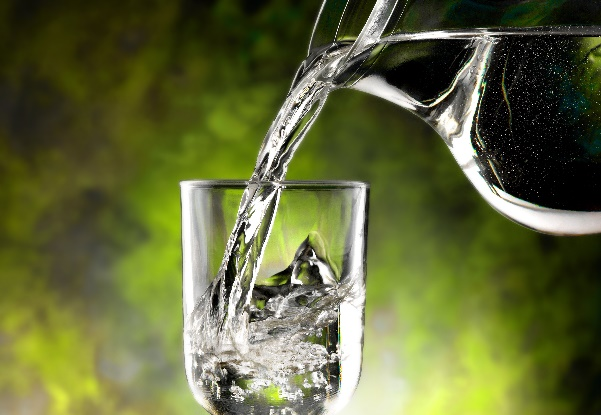
\includegraphics[height=0.225\textwidth]{figures/template_figs/title_img_1}
                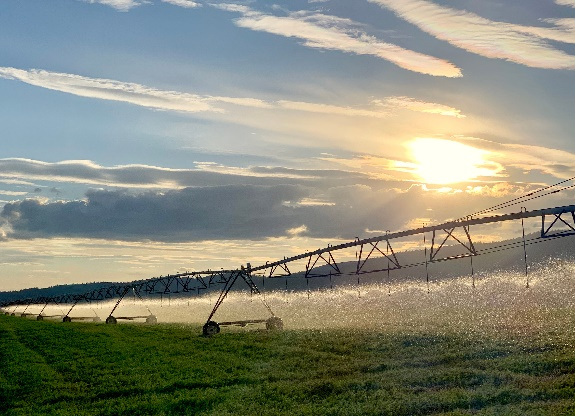
\includegraphics[height=0.225\textwidth]{figures/template_figs/title_img_2}
                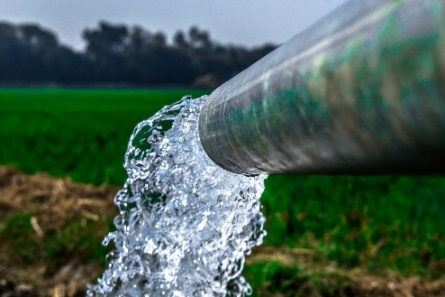
\includegraphics[height=0.225\textwidth]{figures/template_figs/title_img_3}
            \end{center}

        \end{tcolorbox}

        \vspace*{1.5cm}

        \center
        \begin{tcolorbox}[colback=kslvlblue,colframe=ksldarkblue,
            width=0.90\textwidth, valign=center]
            \color{ksldarkblue}
            \textit{Report No: \projcode{}.\nthreport}

            \huge\textbf{\reporttitle{}}

            \normalsize
            \begin{addmargin}[1em]{2em}
                \textit{\normalsize\reportenddate{}}

                \textit{Prepared by Kōmanawa Solutions Ltd. for \client{}}
            \end{addmargin}
        \end{tcolorbox}


        \vfill

        %bottom box
        \begin{center}
            \begin{tcolorbox}[colback=black!80!white,colframe=black!80!white,
                valign=center]
                \color{white!95!brown}
                \huge \textbf{Komanawa.com} \hfill
                
\includegraphics[width=.10\textwidth]{figures/template_figs/just_symbol}

            \end{tcolorbox}
        \end{center}

    \end{center}
\end{titlepage}

%---------------------------------------------------------------------------------------
% footer/header
%---------------------------------------------------------------------------------------
    \pagestyle{fancy}
    \fancyhead{}\fancyfoot{}
    % header
    \fancyhead[L]{
\includegraphics[width=18mm]{figures/template_figs/ksl_for_latex_justlogo}}
    % footer
    \renewcommand{\footrulewidth}{0.4pt}
    \fancyfoot[L]{\textbf{\thepage}~\textbar~KSL}
    \fancyfoot[R]{\truncate[...]{0.75\linewidth}{\reporttitle}}
    \pagenumbering{roman} % set page numbering to roman numerals for intro pages

    % About page
    %! Author = matt_dumont
%! Date = 4/12/23

\color{ksldarkblue} \LARGE \textbf{Kōmanawa:}
\color{black} \large
\begin{enumerate}
    \item (verb) to spring, well up (of water)
    \item (verb) to spring, well up (of thoughts, ideas)
\end{enumerate}
\normalsize

Kōmanawa Solutions Limited (KSL) is a water resource consultancy and research company specialising in water resource investigation and modelling, environmental limit setting and water resource impact assessment. Our goal is to provide excellent science to facilitate the robust management of natural resources in our changing climate. Clients include New Zealand enterprises in the private sector, central and local government agencies and community groups.
Our vision
KSL delivers high quality science and research. We aspire to be at the forefront of creativity and innovation to address our increasingly complex water resource challenges; mō tatou, ā, mō kā uri ā muri ake nei (for us and our children after us).

\color{ksldarkblue} \LARGE \textbf{Our mission}
\color{black} \normalsize

Our mission is to develop solutions to the increasingly challenging water resource management issues we now face by providing a clear vision of the pathway from problem to solution. We work closely with our partners, communities, and stakeholders, deploying state-of-the-art scientific methods and building trust through knowledge and honest science communication.

\color{ksldarkblue} \LARGE \textbf{Limitations}
\color{black} \normalsize

Kōmanawa Solution Ltd (KSL) has prepared this Report in accordance with the usual care and thoroughness of the consulting profession for the use of \client{}.

This Report has been prepared in accordance with the scope of work and for the purpose outlined at the start of this report and is based on generally accepted practices and standards at the time it was prepared. No other warranty, expressed or implied, is made as to the professional advice included in this Report.

Where this Report indicates that information has been provided to KSL by third parties, KSL has made no independent verification of this information except as expressly stated in the Report. KSL assumes no liability for any inaccuracies in or omissions to that information.


This Report was prepared between \reportstartdate{} and \reportenddate{} and is based on the conditions encountered and information reviewed at the time of preparation. KSL disclaims responsibility for any changes that may have occurred after this time.

This Report should be read in full. No responsibility is accepted for use of any part of this Report in any other context or for any other purpose. This Report does not purport to give legal advice. Legal advice can only be given by qualified legal practitioners.

This Report has been prepared for the exclusive use of \client{} and their authorised agents. Except as required by law, no third party may use or rely on this Report unless otherwise agreed in writing by KSL.

To the extent permitted by law, KSL expressly disclaims and excludes liability for any loss, damage, cost or expenses suffered by any third party relating to or resulting from the use of, or reliance on, any information contained in this Report. KSL does not admit that any action, liability or claim may exist or be available to any third party.

\newpage

\color{ksldarkblue} \LARGE \textbf{Version Control}
\color{black} \normalsize

% add version control table
%! Author = matt_dumont
%! Date = 7/12/23

\begin{table}[!ht] % !ht = here or top of page
    \label{tab:vc_table}
    \begin{ksltable}[
    ]{
        colspec = {|m{0.12\textwidth}|m{0.12\textwidth}|m{0.70\textwidth}|},
    }
        Date & Status & Comment \\
        % example row
        07/12/2023 & Draft & This is a dummy comment that goes for a really really really long time to see how this impacts the table \\
        % a couple of empty rows
        ~ & ~ & ~ \\
        ~ & ~ & ~ \\
        ~ & ~ & ~ \\
    \end{ksltable}
\end{table}

\color{ksldarkblue} \LARGE \textbf{Authors}
\color{black} \normalsize

\authors


% contributors empty file is ok here
%! Author = matt_dumont
%! Date = 4/12/23

\color{ksldarkblue} \LARGE \textbf{Contributors}
\color{black} \normalsize

This work was partially funded and supported by the Our Land and Water National Science Challenge project Monitoring Freshwater Improvements (https://www.monitoringfreshwater.co.nz/). In particular, we would like to thank:
\begin{itemize}
    \item \textbf{Olivier Ausseil} - \textit{For providing is expert guidance and steering throughout the our land and water project.}
    \item \textbf{Richard McDowell} - \textit{For his support in the development of the methodologies used in this project.}
\end{itemize}


% box with suggested citation auto generated from doc info
\begin{breakawaybox}[label={box:sugcite}, title=Suggested Citation, flushleft title]
    \textbf{\authorcite{}},
    (\getYear{\reportenddate}). \textit{\reporttitle{}}.
    Report: \projcode{}.\nthreport{} prepared by Kōmanawa Solutions Ltd for \client.
\end{breakawaybox}

\newpage

    % executive summary
    %! Author = matt_dumont
%! Date = 4/12/23
\phantomsection % add to toc (make the link go to the right location)
\addcontentsline{toc}{section}{Key Findings} % add to toc
\section*{Key Findings} \label{keyf} % the asterisk prevents a section number from being assigned

\begin{breakawaybox}[label={box:keyfind}, title=Key Findings]{}
    Our key findings are:
    \begin{itemize}
        \item The current monitoring programme is not well suited to detecting reductions in nitrate at the scale required by \gls{pc1}. Note that this is only one aspect of the monitoring programme and our findings do not comment on the overall quality of the programme.
        \item It will likely be 30 or more years before \gls{pc1} reductions can be detected by the current monitoring regime.
        \item If we incorrectly ignore \gls{no3n} noise and only consider \gls{mrt} (e.g, lag) then the \gls{pc1} reductions should be detectable much sooner (< 15 years for many sites).
        \item The ultimate \gls{no3n} concentration (once all the \gls{no3n} has made it to the sampling point) and the ability of the surface water features to detect changes in \gls{no3n} is highly sensitive to the assumed \gls{mrt}.
        \item Obtaining water age data for all key monitoring sites, particularly in surface water courses, is a key recommendation.
        \item There is a trade-off between the scale of \gls{no3n} mitigations and the cost of the monitoring programme required to detect the effectiveness of these mitigations. Very large mitigations are easy to detect, but may not be realistic for other reasons. Smaller mitigations are typically more tenable, but require a more expensive monitoring programme to detect.
        \item This report demonstrates that bespoke monitoring programmes may often be required to assess the effectiveness of a plan change. We suggest that analysis of the monitoring programme needed and its cost should be an integrated component of the plan change itself.
        \item Finally, detecting \gls{pc1} or similar changes requires a significant investment in monitoring infrastructure and data collection.
    \end{itemize}

\end{breakawaybox}

\newpage

\glsresetall  % reset the glossary acronyms
\phantomsection % add to toc (make the link go to the right location)
\addcontentsline{toc}{section}{Executive Summary} % add to toc
\section*{Executive Summary} \label{exsum} % the asterisk prevents a section number from being assigned


\gls{pc1} of the Canterbury Land and Water Regional Plan included requirements for farmers in the Selwyn Waihora catchment to reduce nitrate discharges to groundwater to support water quality improvements.
\gls{pc1} became operational in 2016 with a requirement for \gls{no3n} reductions to be fully implemented by 2022.
Very few monitoring sites in the Selwyn Waihora catchment and assessed by this report show decreasing \gls{no3n} concentrations to date.
This study evaluates the change detection power analysis of 56 sites (46 groundwater wells and 10 surface water features) to identify when and if \gls{pc1} reductions might become detectable in the current monitoring programme.

\begin{wrapfigure}{R}{0.50\textwidth}
    \begin{breakawaybox}[title=What is Detection Power]{}

        Essentially, detection power describes the chance that you can see whether concentrations are changing over time.
        More specifically, detection power is the percent probability of detecting a statistically robust trend in the receptor concentration time series.
        Noisy data reduces the detection power while more frequent sampling increases the detection power.
        \\
        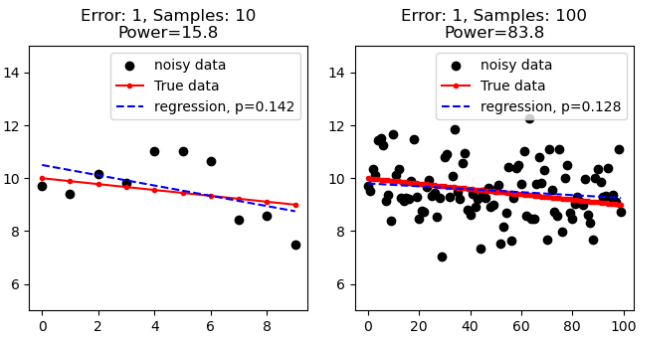
\includegraphics[width=0.99\textwidth]{figures/dp_ex_small}
    \end{breakawaybox}
\end{wrapfigure}

Our analysis suggests that the current monitoring programme is not well suited to detecting reductions in nitrate at the scale required by \gls{pc1}.
\gls{pc1} requires nitrate load reductions between 2-30\% depending on land use (see \autoref{box:no3_red}).
Here we assume at a 20\% reduction in nitrate loads is equivalent to a 20\% reduction in leachate nitrate concentrations; however changes in coincident land surface recharge (e.g., the move to efficient irrigation), could yield lower than expected reductions in nitrate leachate concentrations.
Our analysis suggests that only approximately 60\% of groundwater monitoring sites will ever show decreasing \gls{no3n} concentrations (negative slope) if nitrate concentrations in source soil drainage reduce by 10-20\%.
The remaining 40\% of sites are likely to plateau and larger reductions would be required to observe decreasing concentrations.
Note that these steady state concentrations will be lower than if \gls{pc1} had not been implemented.
The impact of \gls{pc1} on these \say{plateau} sites will not be detectable via slope monitoring (looking for a decreasing concentration trend), but future work may be able to detect these changes using a counterfactual approach (i.e., asking whether the \gls{no3n} concentration is significantly different to the concentration without reductions).
There is significant uncertainty in these estimates due to the lack of \gls{mrt} data in c. 60\% of the groundwater monitoring locations we investigated.
However, if our \gls{mrt} estimates are correct then the nitrate reductions required under \gls{pc1} should be detectable in c. 30\% of the monitoring wells (50\% of those which can have a decreasing trend) by c. 2060.
Increasing sampling frequencies to monthly or weekly would allow detection of the reductions in c. 30\% of the monitoring wells by 2040 or 2035, respectively.

Surface water features generally receive water from a much larger catchment than individual wells and are therefore more likely to provide a landscape scale representation of policy and land management action effectiveness.
However, no water age data are available for surface water courses in the Selwyn Waihora catchment, making robust predictions of change detection power impossible.
We therefore derived detection power estimates by assuming a range of \gls{mrt} values.
Our results show that the detection power of the surface water features is highly sensitive to the assumed \gls{mrt} value.

As an example, our analysis of Hart's creek highlights the uncertainty associated with our assumed water ages.
Results indicate that the maximum steady state \gls{no3n} concentration could be as low as 7.6 mg/l (assuming a \gls{mrt} of 5 years) or could be as high as 12.0 mg/l (assuming a \gls{mrt} of 30 years).
A stated goal of \gls{pc1} was to set an annual limit across all the shallow groundwater of not more than 8.5 mg/L.
The Hart's creek results may indicate that the \gls{pc1} reductions are sufficient to achieve this goal, or that the reductions are insufficient to prevent shallow groundwater from exceeding the \gls{mav} in drinking water (11.3 mg/L).
Obtaining age data for the surface water network would constrain these predictions and allow integrated analysis of detection power across the groundwater and surface water monitoring programme.
The programme could then be optimised in terms of the number and location of sites and monitoring frequency for change detection power, spatial representativeness and monitoring cost.
Age data collection for surface watercourses would also help to constrain the likely maximum \gls{no3n} concentration in a stream that will arise from current and past land use; this will provide a much clearer picture of policy and land management actions required to achieve water quality objectives.

We conclude that the current groundwater monitoring programme is unlikely to detect whether the nitrate reductions mandated under \gls{pc1} have improved water quality within the timeframes required for effective water resource management (within 30 years or less).
Previous analysis has focused on lag times as the key constraint on detecting change, but this analysis shows that statistical power is an equally important constraint under the current sampling frequency.
We recommend that the change detection monitoring design framework described in the \textit{\href{https://github.com/Komanawa-Solutions-Ltd/gw_detect_power/blob/main/supporting_documents/Water_quality_monitoring_for_management_of_diffuse_nitrate_pollution_Final.pdf}{Water quality monitoring for management of diffuse nitrate pollution report}} \citep{olw_guidance}
should be applied to improve the surface water and groundwater monitoring programme for change detection. Key tasks will include:
\begin{itemize}
    \item Obtaining water age data for all key monitoring sites, particularly in surface water courses.
    \item Developing a basic conceptual model of the spatial distribution and rate of expected nitrate loss reductions, water flow paths, potential attenuation and travel times.
    \item Carrying out an integrated analysis of groundwater and surface water detection power for existing sites in the monitoring area using the information provided in this report, updated with new water age data where required, and identifying the highest detection power sites.
    \item Evaluating the representativeness of high power monitoring sites in relation to the expected spatial distribution and distribution of nitrate loss reductions and the number of sites required to confidently detect change.
    \item Identify new monitoring sites if existing network detection power and/or representativeness is inadequate.
    \item Undertaking a sampling frequency cost-benefit analysis.
    \item Undertaking more sophisticated statistical analysis to extract additional information from the existing data.
    \item Finalising network and monitoring design.
    \item Reviewing data after 1, 3 and 5 years of sampling to determine whether detection power and timeframe requirements have changed in light of new information.
\end{itemize}

We note that these recommendations will require a significant investment in monitoring infrastructure and data collection. A companion study found that a 100-300\% increase in investment is likely required nationally to meet these goals \citep{dumont_determining_nodate}.
This highlights the discrepancy between the goals of national monitoring programmes and the resources available to regional councils to meet these goals.
This can be further exacerbated by the desire for smaller or more gradual interventions; the larger the change in \gls{no3n} the easier it is to detect that change.
This is a national challenge for regional councils and communities across New Zealand.

A key caveat of this report is that we only focused on one aspect of the monitoring programme: detecting changes in \gls{no3n} concentrations.
The network serves and was primarily designed for multiple other purposes some of which are counter to high detection powers (e.g., characterising the state of the deep aquifer system).
We also have not assessed the spatial representativeness of the monitoring network in this analysis (for either change detection or more broadly) as it was beyond the scope of this project.
    \newpage

%---------------------------------------------------------------------------------------
%%	Table of contents SECTIONS
%---------------------------------------------------------------------------------------

    % Table of contents
    \phantomsection % add to toc (make the link go to the right location)
    \addcontentsline{toc}{section}{Contents} % add to toc
    \tableofcontents

    % toc of figures
    \phantomsection % add to toc (make the link go to the right location)
    \addcontentsline{toc}{subsection}{List of Figures} % add to toc
    \listoffigures

    % toc of tables
    \phantomsection % add to toc (make the link go to the right location)
    \addcontentsline{toc}{subsection}{List of Tables} % add to toc
    \listoftables

    % TOC of breakaway boxes based on last entry of
    %    https://tex.stackexchange.com/questions/86711/tcolorbox-list-of-listings
    \phantomsection % add to toc (make the link go to the right location)
    \addcontentsline{toc}{subsection}{Table of Breakaway Boxes} % add to toc
    \tcblistof[\section*]{bab}{List of Breakaway Boxes}

    % List of abbreviations/definitions
    \addcontentsline{toc}{subsection}{Definitions and Abreviations} \label{sec:defs}
    \printglossary[title=Definitions and Abreviations, nonumberlist]

    \newpage

%---------------------------------------------------------------------------------------
% footer/header
%---------------------------------------------------------------------------------------
    % add more to the header
    \fancyhead[C]{\leftmark}
    \fancyhead[R]{\rightmark}
    \setcounter{page}{1} % reset page counter
    \pagenumbering{arabic} % set page numbering to arabic numerals for main pages

   \glsresetall % reset glossary counts at the start of the main text
%---------------------------------------------------------------------------------------
    % custom_sections
%---------------------------------------------------------------------------------------
    %! Author = matt_dumont
%! Date = 14/12/23

\section[Introduction]{Introduction} \label{sec:intro}

\gls{no3n} is a contaminant of significant concern both worldwide and in Aotearoa / New Zealand.
At concentrations > 0.8 mg/l, \gls{no3n} can stimulate the growth of periphyton and phytoplankton \citep{mcdowell_global_2020}; concentrations greater than 2.4 mg/l can cause toxicological effects to in stream fauna \citep{camargo_nitrate_2005, horak_assessing_2019,wagenhoff_identifying_2017};
finally concentrations above the \gls{mav} (>11.3 mg/l) can cause human health impacts \citep{rahman_anthropogenic_2021}.

\begin{wrapfigure}{R}{0.5\textwidth}
    \begin{breakawaybox}[label={box:no3_red}]{Plan Change 1}
        \textbf{Objective:} Reduce \gls{no3n} concentrations in the Selwyn Waihora zone to reduce the load to Te Waihora / Lake Ellesmere and ensure that average groundwater \gls{no3n} concentrations are not more than 8.5 mg/L.\\

        \gls{no3n} reductions required by \glsfirst{pc1} vary by land use:
        \begin{itemize}
            \item 30\% for dairy
            \item 2\% for dryland sheep, beef or deer
            \item 22\% for dairy support
            \item 7\% for arable
            \item 20\% for pigs
            \item 5\% for fruit, viticulture or vegetables
            \item 5\% for irrigated sheep, beef or deer
        \end{itemize}

        Note that these reductions are applied to the \gls{no3n} load.
        We assume that a \gls{no3n} load reduction is equivalent to a \gls{no3n} concentration reduction, but changes land surface recharge (e.g., the move to efficient irrigation), could yield lower \gls{no3n} concentration reductions.
    \end{breakawaybox}
\end{wrapfigure}

The Selwyn Waihora zone is a large catchment in the Canterbury plains south of Christchurch.
The catchment stretches from the foothills of the Southern Alps to the coast.
There is significant agricultural activity, as well as many high value ecosystems including Te Waihora / Lake Ellesmere and the Kaitorete Spit.
The Selwyn Waihora zone is also home to many significant cultural sites for Ngāi Tahu, the local iwi.
\gls{no3n} concentrations in the Selwyn Waihora zone are elevated with many surface water sites exceeding the \gls{natbotno3} of 2.4 mg/l \citep{noauthor_national_2020}.
\gls{pc1} of the Canterbury Land and Water Regional Plan, operative from 1st February 2016, includes provisions to reduce nitrate leaching concentrations in the Selwyn Waihora; however there was acknowledgment \gls{no3n} concentrations could initially continue to increase after implementing \gls{pc1} reduction.
In addition, \gls{pc1} predated the National Policy Statement for Freshwater Management 2020 and therefore the \gls{natbotno3} of 2.4 mg/l was not a requirement of \gls{pc1}.
\gls{pc1} \gls{no3n} reductions ranged from 2-30\% \autoref{box:no3_red}.
Implementation of these \gls{no3n} reductions were expected to begin in 2017 and should have been fully implemented by 2022.


Environment Canterbury maintains a network of monitoring wells and surface water sites to track \gls{no3n} concentrations in the Selwyn Waihora zone as is required by the The Resource Management Act 1991.
The monitoring programmes are reviewed periodically with the most recent review of the groundwater quality and water level network being in 2022.
The state purpose of the groundwater monitoring programme is to:
\begin{itemize}
    \item Monitor long-term groundwater state and trends.
    \item Improve scientific understanding of Canterbury groundwater systems and help Environment Canterbury manage groundwater in the region.
    \item Assess progress against freshwater outcomes.
    \item Inform the effectiveness of regional policies and plans \citep{ecan_monitor_review}.
\end{itemize}

Although many landowners have stated they have already fully implemented the required reductions \citep{scottpc}, \gls{no3n} concentrations at most sites in the Selwyn Waihora zone have not yet shown any significant reductions \citep{ecan_annual_survey}.
This discrepancy could be caused by a number of factors including:
\begin{itemize}
    \item Lag
    \begin{itemize}
        \item \gls{no3n} concentrations have not yet reached steady state with the monitoring network.
        \item Historical increases in \gls{no3n} concentrations that have yet to reach steady state with the monitoring network.
        \item \gls{no3n} stored in the unsaturated (vadose) zone.
    \end{itemize}
    \item Insufficient precision in the \gls{no3n} monitoring programme (a lack of detection power).
    \item Nitrate loss mitigations are less effective than expected.
    \item The difference in \gls{no3n} load and \gls{no3n} leachate concentration. \gls{pc1} reductions are defined as percent reductions in \gls{no3n} load. Changes in coincident land surface recharge changes (e.g., more efficient irrigation) can yield increasing or decreasing \gls{no3n} leachate concentration.
    \item Poor or incomplete implementation of on-farm mitigations.
    \item Other factors such as climatic variations and boundary condition changes (e.g., changes in losses from leaky water races) impacting groundwater recharge.
\end{itemize}

The purpose of this study is to better understand:
\begin{enumerate}
    \item when the implemented reductions should be observable in the current monitoring programme
    \item obstacles to detecting \gls{no3n} reductions in the Selwyn Waihora zone.
\end{enumerate}

We focus on the potential statistical errors that can arise from the monitoring programme design.
The monitoring programme detecting a trend when none is present (Type I error), failing to detect a real trend (Type II error), or estimating a trend that is opposite to the one present (Type III error); could affect any management decisions based on the monitoring results could undermine rather than support the management objectives.

    %! Author = matt_dumont
%! Date = 14/12/23

\section[Methods]{Study Methodology}   \label{sec:methods}

\subsection[Data]{Receptors, Data processing, and analysis} \label{sec:data}

\gls{ecan} provided us with \gls{no3n} concentration data for approximately 100 sites which included groundwater monitoring wells, spring fed streams and the Selwyn Waikirikiri River at Coes Ford. The Selwyn Waikirikiri River has both hill fed and spring fed components, but in the lower catchment it is a gaining stream and the low flows are dominated by spring fed flow. We worked collaboratively with \gls{ecan} to select a subset of sites for analysis (\autoref{fig:sitelocs}). The raw data and all outputs are available in the \gls{proj_repo} and a summary table of the data is available in \autoref{appx:data} Groundwater age data (\gls{mrt} and age distribution parameters) were provided by both \gls{ecan} and \gls{olw}.

\begin{landscape}
    \kslfig{0.95\textwidth}{../figures/selwyn_sites}{Final Site Locations}{sitelocs}
\end{landscape}

The data was processed as follows:
\begin{enumerate}
    \item \textbf{\gls{no3n} Outlier Identification}: we identified two types of outliers (see \autoref{fig:ex_outlier_trend}):
    \begin{enumerate}
        \item  True outliers: values which based on a statistical and visual analysis were clearly outside the expected range of values for the site. These values were removed from the dataset.
        \item Trend outliers: data which precede the most recent / current trend and could erroneously affect the fit of the current historical trend. These values were not included in the historical trend analysis or \gls{no3n} noise estimation.
    \end{enumerate}
    \item \textbf{Estimate the age distribution, wells}: where sites did not have assessed groundwater age distributions we estimate the parameters from nearby sites. The method was somewhat manual and was often site specific. Details on how we estimated the age distribution for each site are available in the \gls{proj_repo}.
    \item \textbf{Estimate the age distribution, streams}: There were no age estimates for the spring fed streams; therefore we assessed the detection power assuming a range \gls{mrt}, 5, 10, 20, and 30 years. The other age model parameters were assumed to be the median of all sites within (7.5 or 10 km) and <=10m depth. Further details are available in the \gls{proj_repo}
\end{enumerate}

\kslfig {0.90\textwidth}{figures/m36_8187}{Site M36/8187: note the "true" outliers (black) and the trend outliers(red)}{ex_outlier_trend}


\subsection[Pathways]{\textit{A. priori} Pathways} \label{subsec:apriori}

In consultations with \gls{ecan} we generated the following \textit{a. priori} pathways for the implementation of \gls{no3n} reductions:
\begin{itemize}
    \item \textbf{No change}: no change in \gls{no3n} source concentrations.
    \item \textbf{5\% reduction}: a 5\% reduction in \gls{no3n} source concentrations implemented linearly between 2017 and 2022.
    \item \textbf{10\% reduction}: a 10\% reduction in \gls{no3n} source concentrations implemented linearly between 2017 and 2022.
    \item \textbf{20\% reduction}: a 20\% reduction in \gls{no3n} source concentrations implemented linearly between 2017 and 2022.
    \item \textbf{30\% reduction}: a 30\% reduction in \gls{no3n} source concentrations implemented linearly between 2017 and 2022.
\end{itemize}

While \gls{pc1} specifies the reductions, it does not apply to all land parcels. The source zones for many wells and spring fed streams are poorly constrained. Providing multiple pathways provides an efficient mechanisms to explore the potential impact of different source zones and mitigation effectiveness. A higher than expected reduction pathway was provided to explore the potential impact of a more effective than expected implementation of \gls{pc1}.

\subsection[Detection Power Methods] {Detection Power Methods} \label{subsec:detection_power_methods}

The method to calculate the detection power of a given site was implemented after % todo cite my paper
using our open source package. % todo cite my package
Briefly the methodology is as follows for each site:
\begin{enumerate}
    \item Ascertain whether the historical concentration data has a statistically robust trend (e.g. via a Mann-Kendall test, see \autoref{fig:ex_outlier_trend})
    \item Estimate the noise in the receptor concentration time series
    \begin{enumerate}
        \item If the historical concentration data has an increasing statistically robust trend, then the noise can be estimated as the standard deviation of the residuals from a model (e.g. a linear regression or Sen-slope/ Sen-intercept).
        \item If the historical concentration data does not have a statistically robust trend, then the noise can be estimated as the standard deviation of the receptor concentration time series.
        \item If the historical concentration data has a statistically robust decreasing trend, we assumed that the receptor was at steady state and considered the site in the same fashion as a site with no statistically robust trend.
    \end{enumerate}
    \item Estimate the source concentration from the historical trend (if any) and the groundwater age distribution.
    \item Predict the true receptor concentration time series (e.g., the concentration at the receptor if there was no noise) based on the aforementioned source concentration, \textit{a priori} pathway and the groundwater age distribution.
    \item Resample the true receptor concentration time series to the desired sampling frequency and duration (e.g., quarterly sampling for 10 years).
    \item Calculate the statistical probability of detecting the change
    \begin{enumerate}
        \item generate a synthetic sample of the receptor noise (e.g., by sampling a normal distribution)
        \item add the synthetic noise to the true receptor concentration time series
        \item conduct a statistical test (here we used a Mann-Kendall test or a Multipart Mann Kendall test) to determine if the synthetic receptor concentration time series has a statistically robust trend
        \item repeat steps a-c many times (we used 1000 iterations). The probability of detecting the change is the number of times the synthetic receptor concentration time series had a statistically robust trend divided by the number of iterations.
    \end{enumerate}
\end{enumerate}

The source concentration was estimated by fitting a simple source to receptor model. The source concentration was set via a parameterised trend and minimum value and then the source concentration was transformed to the receptor concentration via the \gls{epfm}. \autoref{fig:source_ex} provides an example of the source concentration estimation. Site M36/0698 has a statistically robust increasing trend, approximate 0.12 mg/l \gls{no3n}. Given the \gls{mrt} of 22.75 years the best fit of the data (solid gold line) suggests that the peak source concentration is likely c. 7 mg/l \gls{no3n} (dashed gold line). More details on this process are available in % todo cite my paper  and gw age tools repos

\kslfig {.95\textwidth}{figures/m36_0698_red20_true_conc}{Site M36/0698 as an example of the source concentration prediction}{source_ex}

For the statistical test we used:
\begin{itemize}
    \item A \textbf{Mann-Kendall test} for sites without a historical increasing trend
    \item A \textbf{Multipart Mann-Kendall test} for sites with a historical increasing trend. We used a Multipart Mann-Kendall test here as a historically increasing trend can continue after the implementation of \gls{pc1}, due to historical increases in \gls{no3n} source concentrations which have not reached steady state at the receptor. A traditional Mann-Kendall test would require the absolute knowledge of the time of the maximum \gls{no3n} receptor concentration. A Multipart Mann-Kendall test does not require this knowledge. For more information see % todo cite my mpmk repo
\end{itemize}

We set the critical level at 5\% (<0.05) for both tests. For the Mann-Kendall test this means that the trend was detected if p<0.05. For the multipart Mann-Kendall test this means that the trend was detected if there was any breakpoint where the older data was increasing (p<0.05) and the newer data was decreasing (p<0.05). Note that a minium of 5 datapoints were required for each part in the multipart Mann-Kendall test. Finally, some sites would not have a decreasing \gls{no3n} concentration because the implemented reduction were not sufficient to reduce steady state concentrations below the current level. In this case the aforementioned multipart Mann-Kendall test would never detect the trend. Therefore, we conducted a subsequent multipart Mann-Kendall test which identified a breakpoint where there was an earlier increasing trend (p<0.05) and subsequently no trend (p>0.5). These Plateau sites are further discussed in \autoref{sec:plateau_results}.


    %! Author = matt_dumont
%! Date = 14/12/23

\section[Results and Discussion]{Results and Discussion} \label{sec:results}

%--------------------------------------------------------------------------------------------------------------
\subsection[Site Results]{Results for Individual Sites} \label{sec:site_results}

Although we have produced results and figures for each site, it is beyond the scope of this report to discuss the detection power of each site; however all figures are available in the \gls{proj_repo}.
An example of the individual site detection power plots is shown in \autoref{fig:ex_plot}.
The figure details the detection power of site M36/3588 assuming a 30\% reduction in nitrate concentrations.
There are two subplots; for both the x-axis is the sampling duration/date.
For the top plot the y-axis is \gls{no3n} concentration (mg/l).
The raw sample data and whether those data were included in the analysis (blue included, red/black not included), the predicted source concentration (yellow), the predicted receptor concentration with (gold) and without the implemented reduction (fuchsia) are all plotted.
In the lower subplot the y-axis depicts the likelihood that a change in nitrate concentrations will be detected.
The color of the line represents the sampling frequency (e.g. monthly, quarterly, etc.).
Note that the black/grey line is the detection power assuming that the receptor has no \gls{no3n} noise.
Effectively, the grey line is when the change would be detected if only lag was considered.
The correct interpretation of this plot is that the lag at this well only allows a theoretical change detection at or after 2027 (grey line).
However, if we consider the obscuration of noise, then with quarterly sampling the detection power is only likely to exceed 80\% in 2037 (gold line).
We use the cutoff of 80\% as it is typically used nationally and internationally as the acceptable threshold for confidently drawing conclusions and/or making decisions from the monitoring results interpretation\citep{dumont_determining_nodate}.

\kslfig {0.95\textwidth}{../GeneratedData/power_calc_site_plots/m36_3588_red30}{An example of the individual site detection power plots}{ex_plot}{}

%--------------------------------------------------------------------------------------------------------------
\subsubsection[Plateau Sites]{Plateau Sites: Sites Where \gls{no3n} Concentrations Will Not Decrease Under the assumed Pathway} \label{sec:plateau_results}

%! Author = matt_dumont
%! Date = 16/12/23
\begin{wraptable}{R}{0.4\textwidth}
    \centering
    \caption{Percent of the groundwater network that will level off but never show a decreasing trend in the receptor at a theoretical reduction level at the source}
    \label{tab:plateau}
    \begin{ksltable}[
    ]{
        colspec = {|c|c|},
    }
        Reduction & Plateau sites \\
        5\% & 57\% \\
        10\% & 48\% \\
        20\% & 33\% \\
        30\% & 9\% \\
    \end{ksltable}
\end{wraptable}

Some sites will not show a statistically robust decreasing trend under the assumed pathway.
We refer to these sites as plateau sites. An example of a plateau site is shown in \autoref{fig:ex_plateau}.
Well L35/0205 is a plateau site because the steep increasing trend in concentration in combination with the significant \gls{mrt} suggest that the source and receptor concentration are at a significant disequilibrium.
Therefore, the rather minor reductions (10\%) in the assumed pathway will simply lower the eventual steady state concentration (e.g., gold vs fuchsia lines), but will not reduce the concentration below the observed initial concentration (sen slope fit in 2017).


These plateau sites can cause a significant challenge in detection of nitrate leaching reductions.
Our knowledge of equilibrium nitrate concentrations in the absence of nitrate loss reductions is poor.
This makes it difficult to understand the cause of any difference between a future observed steady state concentration (once concentration levels off) and the predicted steady state concentration (e.g., the fuchsia line in \autoref{fig:ex_plateau}).
The differences could be due a number of factors \autoref{sec:intro} as well as, on the ground actions not actually being implemented and/or inaccuracies in the estimate of steady state concentration.
These sites will require more sophisticated statistical analysis (for instance a counter-factual approach) to determine whether the \gls{pc1} nitrate loss reductions have been implemented.

\autoref{fig:plateau_locs} shows the location of these plateau sites and the required reduction to yeild a decreasing \gls{no3n} slope in the receptor.
Note we did not include the surface water features here as there is too much uncertainty surrounding their \gls{mrt}.
For the red shaded sites nitrate concentrations would only expect to decline in the well if the average nitrate loss reduction in the monitoring well capture zone is greater than 5\% otherwise the \gls{no3n} concentrations will plateau at a lower level than if no reductions had occurred.
If an average nitrate loss reduction of 10\% is assumed, nitrate concentrations in the fuchsia, gold and blue shaded sites would all plateau at some point in the future, with no measurable decrease occurring.
\autoref{tab:plateau} shows the percent of the groundwater network that will not show a decrease in \gls{no3n} concentrations at a given reduction level in the source.
For example, 57\% of the groundwater network will not show a decrease in \gls{no3n} concentrations if the source is reduced by 5\%.
This suggests that the \gls{pc1} reductions may not yield steady state concentrations below 2017 concentrations for a significant portion of groundwater network; however this is not necessarily a failure of \gls{pc1} as concentrations were expected to continue to increase after the implementation of \gls{pc1}, but to achieve an average concentration of <8.5 mg/l.

\kslfig {.95\textwidth}{../GeneratedData/power_calc_plateau_sites/l35_0205_red10}{An example of a Plateau Site}{ex_plateau}{}

\begin{landscape}
    \kslfig {1.25\textwidth}{../GeneratedData/geospatial_plots/plateau_locs}{The \gls{no3n} reductions needed at which a given site to yield a negaitve slope rather than a lower steady state concentration (wells only)}{plateau_locs}{}
\end{landscape}

%--------------------------------------------------------------------------------------------------------------
\subsection[Mean Residence Time Impacts]{Mean Residence Time, Steady State Concentration, and Detection Power} \label{sec:mrt_results}

\begin{wrapfigure}{R}{0.5\textwidth}
    \begin{breakawaybox}[
        label={box:wierdresults}]{Counterinuitive Results}
        Some of the results here are counterintuitive; for instance, in \autoref{fig:sw_mrt} the detection power is higher with a \gls{mrt} of 10 years than with a \gls{mrt} of 5 years. Additionally, for some receptors (not pictured) the detection power increases and then subsequently decreases with increasing sampling duration.

        This odd behaviour is due to the statistical method used. Fundamentally we are fitting a Mann-Kendall to the data and specifying success as p<0.05. A rapid change (low lag and/or a swift implementation period) pared with infrequent sampling can lead to the receptor reaching steady state before the statistical test can confidently detect the reduction. The ensuring long flat period, where the true receptor concentration is not changing, leads to a higher p-value in the statistical test and therefore lower detection power. In these instances another statistical test (e.g., a counterfactual approach), maybe a more robust method to detect the change. This is discussed in \autoref{sec:counterfactual}.
    \end{breakawaybox}
\end{wrapfigure}

Our use of a set of indicative \gls{mrt} values for surface water features demonstrates the impact that uncertainties in the age distribution impacts both detection power of a receptor, and it's steady state \gls{no3n} concentrations.
\autoref{fig:sw_mrt} demonstrates the impact of the assumed \gls{mrt} on the estimation of the steady state \gls{no3n} concentration in Harts Creek.
Harts creek is a small spring-fed tributary of Te Waihora (Lake Ellesmere) on the southwestern side of the lake.
There a substantial historical record of increasing \gls{no3n} concentrations, but there are no data on the age of the water within the creek.
Our simple source concentration modelling (see \autoref{subsec:detection_power_methods}) and the measured nitrate concentration data prior to 2017 suggest that the peak steady state concentrations in the receptor (without reductions) could range between 7.6 to 12.0 mg/l \gls{no3n} depending on the \gls{mrt} assumed.
This large range is significant from a water resource management perspective --- the maximum possible value is beyond the drinking water limit.
Concentrations in spring fed streams above the drinking water limit would imply that water supply wells in the catchment are, on average, likely to exceed the limit.
In addition, the nitrate loss reductions required to achieve the national bottom line nitrate concentration in the stream vary widely between these two estimates, which has important implications for farming in the stream catchment (though as noted this threshold postdates \gls{pc1}).

The uncertainty in the likely maximum peak concentration in this receptor could be significantly constrained with one or more relatively cost-effective age tracer samples.
It is also worth understanding that in surface water features \gls{mrt} may not be a static value, but may vary with stream flow with higher flows, where runoff is a higher percentage of the flow, having a younger \gls{mrt} than base flows where more of the stream flow is likely derived from groundwater.

\kslfig {0.95\textwidth}{../figures/mrt_matters.png}{The impact of assumed \gls{mrt} on the steady state \gls{no3n} concentrations and the potential to detect \gls{pc1} reductions (red.)}{sw_mrt}{For example, if \gls{mrt} to the river site is less than 5 years, a decreasing trend would be observed, but if the MRT is 30 years then legacy nitrate will still be in transit and concentrations continuing to increase before they plateau.}

The \gls{mrt} is also a significant factor for detecting \gls{pc1} \gls{no3n} reductions.
If the \gls{mrt} is relatively low (5-10 years) then it would be feasible to detect \gls{pc1} reductions by 2032 with the current (monthly) or slightly higher sampling frequency.
A higher \gls{mrt} of 20 years would significantly reduce detectability and with a \gls{mrt} of 30 years, the \gls{pc1} nitrate loss reductions are unlikely to result in a decrease in \gls{no3n} concentrations (see \autoref{sec:plateau_results}) relative to their 2017 concentrations.
Note that the counterintuitive result that the detection power with \gls{mrt} of 5 years is lower than that of \gls{mrt} 10 years is discussed in \autoref{box:wierdresults}.


%--------------------------------------------------------------------------------------------------------------
\pagebreak
\subsection[Network Detection Power]{Network Level Detection Power} \label{sec:network_results}
\kslfig {0.95\textwidth}{../GeneratedData/geospatial_plots/detect_power_locs_red20_freq4}{Sampling duration until the probability of detecting a reduction is $\geq80\%$ }{timetodetect}{}


\begin{wrapfigure}{R}{0.5\textwidth}
    \begin{breakawaybox}[label={box:sfreq}]{Historical mean well sampling frequency}
        \begin{itemize}
        \item \textbf{Annually - Biannually}: 27 sites
        \item \textbf{Biannually - Quarterly}: 10 sites
        \item \textbf{Quarterly +}: 9 sites
        \item \textbf{46 sites total}
        \end{itemize}
    \end{breakawaybox}
\end{wrapfigure}

\autoref{fig:network20} shows the sampling duration required to detect \gls{pc1} nitrate loss reductions (assuming a full 20\% reduction) with 80\% probability using quarterly sampling.
The black dashed line in \autoref{fig:network4per} shows the percentage of the network which can detect \gls{pc1} reductions assuming that the true receptor concentration (i.e., with no noise) is known.
This analysis includes the effects of lag, but excludes the obscuration of the reductions by \gls{no3n} variability / noise and therefore represents the upper limit of change detection potential for very low (zero) noise sites or at very high sampling frequencies.
\autoref{fig:timetodetect} provides a geospatial representation of \autoref{fig:network20} and the 20\% subplot of \autoref{fig:network4per}.
In combination these figures shows that the vast majority of the groundwater network will not be able to detect \gls{pc1} reductions with quarterly sampling.
Increasing the sampling frequency can significantly increase the detection power of the network, but the detectability is constrained by the lag component - time needs to pass before we can identify the reductions.

These results are consistent with the observation that very few monitored wells in the catchment currently have a statistically significant reducing trend (only 3 of 46 sites in this study, and only 9 of 102 sites for which we were originally provided data by \gls{ecan}).
Given our results, the lack of reducing \gls{no3n} concentrations cannot distinguish whether or not \gls{pc1} reductions have been successfully implemented.
If we assume a full 20\% \gls{no3n} reduction in the all the source zones, them of the 46 groundwater sites in this study only 30 sites will have any decreasing \gls{no3n} concentrations(see \autoref{sec:plateau_results}).
At current quarterly sampling rates, it will likely take until 2062 before 15 sites (50\% of those that we modelled as having decreasing \gls{no3n} concentrations) will have a statistically significant reduction in \gls{no3n} concentrations.
Increasing to weekly or monthly sampling would improve the detection power of the network, and we could expect detection in those 15 sites by 2042 and 2037, respectively.
However, any increase in sampling frequency would require a proportional increase in resource for the monitoring programmes.

\autoref{fig:network4per} shows the effect of different reductions on detection power with a quarterly sampling frequency.
Note that these figures exclude the plateau sites (see \autoref{sec:plateau_results} and \autoref{tab:plateau}).
If we assume 10\% reductions on average in the source zone, then:
\begin{enumerate}
    \item Nearly 50\% of the network wells will never measure a decreasing \gls{no3n} concentration.
    \item With quarterly sampling we would not expect to see evidence of a 10\% reduction in more than 10\% of the remaining network and not until after 2050.
    \item Increasing sampling frequencies to monthly or weekly would significantly improve the probability of detection these changes(\autoref{fig:network10}). Note that increasing sampling frequency will not impact the plateau sites.
\end{enumerate}

\begin{landscape}

    \kslfig {1.25\textwidth}{../GeneratedData/overview_plots/well_detection_overview_red20}{The proportion of the groundwater network whick is likely to detect the full \gls{pc1} reductions (20\%)}{network20}{}

    \kslfig {1.25\textwidth}{../GeneratedData/overview_plots/well_detection_overview_freq4}{The propotaion of the groundwater network which is likely to detect reduction at the current quarterly sampling frequency}{network4per}{}

    \kslfig {1.25\textwidth}{../GeneratedData/overview_plots/well_detection_overview_red10}{The proportion of the groundwater network whick is likely to detect the full \gls{pc1} reductions (10\%)}{network10}{}

\end{landscape}

%--------------------------------------------------------------------------------------------------------------
\subsection[Counterfactual Approach]{The Benefits of a Future Counterfactual Approach} \label{sec:counterfactual}

The analysis presented here is designed to answer the question: \say{How long will it take to detect \textit{any} reduction in \gls{no3n} at our existing receptors?} This is a useful question, but it is not the only question that can be asked.
For example, we could ask: \say{How long will will we need to monitor to determine whether a 20\% concentration reduction has occurred?} or \say{How long before we can determine whether or not we are on track for at least a 10\% \gls{no3n} reduction?}.
These questions require a different statistical approach --- a counterfactual approach.
Essentially, the question answered by a counterfactual approach is: \say{How long until we are confident that pathway 1(e.g. no reduction) and pathway 2(e.g., 10\% reductions) are significantly different?}.
A counterfactual approach has not yet been implemented in the groundwater detection power calculator\citep{dumont_komanawagw_detect_power_2023}, but it is being developed and will be available by mid 2024.
It is worth noting that any uncertainty in the source concentration (i.e., at the base of the root zone), which is typically uncertain, is more likely to yield additional uncertainty in the counterfactual detection power.
This is because the absolute difference between two pathways is important under a counterfactual approach whereas only the relative change is necessary for the `reduction` detection power approach presented in this report.

Finally, it should be noted that neither the approach presented here nor the counterfactual approach can reliably determine whether a specified concentration reduction has occurred: a steady state receptor nitrate concentration at the time the reduction is implemented would be required for this. Depending on the distribution of the water age, it can take significantly longer than the \gls{mrt} for a receptor to reach steady state with current land use.

%--------------------------------------------------------------------------------------------------------------
\subsection[Possible Network Improvements]{How to Improve the Detection Power of the Existing Network}

Our results suggest that the current monitoring programme is unlikely to detect whether the \gls{pc1} \gls{no3n} reductions have been implemented successfully in the short to medium term under the current monitoring frequency.
It may be possible to reduce the monitoring duration required to detect change via bespoke monitoring at new sites with a low \gls{mrt} and low signal/noise ratio.
Of course sufficient sampling, and thus time, would be required at any new site.
Although reducing \gls{no3n} concentrations in such would provide confidence that \gls{no3n} concentrations are going in the right direction (down), the results could not prove that the changes were due to \gls{pc1} because these reductions have, theoretically, already been implemented.
Some young groundwater could already be approaching steady state with respect to the \gls{pc1} nitrate loss reductions.
This means that, depending on the \gls{mrt}, a zero change in concentration could be consistent with successfully implemented \gls{pc1} reductions.

Instead, we suggest that the best approach to improve the unambiguous detection of \gls{pc1} reductions is to:
\begin{enumerate}
    \item Increase the certainty of the \gls{mrt} estimates in groundwater detection network; only c. 30\% of groundwater sites had a \gls{mrt} assessment (e.g., via tritium). The remaining 60\% were estimated from nearby wells, which introduces a significant amount of uncertainty. Further age assessments would significantly improve the certainty of the network's detection power and allow increased frequency sampling to occur at sites which are likely to detect the change.
    \item Increase sampling at selected sites that this analysis (or additional analysis with additional \gls{mrt} assessments) show a suitably high probability of detecting \gls{pc1} reductions.
    \item Similar to 1. the surface water network has a significant amount of information about the catchment and acts as an integrator of water quality from a much larger sample of land within the Te Waihora catchment. This alleviates some of the challenges of the spatial representativeness of the groundwater network\citep{olw_guidance}; however the utility of this information is thwarted by the lack of \gls{mrt} assessments. Understanding the age distribution and the relationship between the age distribution and river/stream stage/flow would unlock the power of these sites and support design of an optimized and integrated water quality monitoring programme.
    \item Finally, more sophisticated statistical analysis could be used to extract more information from the existing data and significantly reduce the time required to determine whether the \gls{pc1} plan rules and associated land management actions are successfully reducing nitrate concentrations.
\end{enumerate}

Importantly, the current network is used for more than just change detection.
In some cases these alternative uses are directly in conflict with change detection.
For instance, if the purpose of the network is to provide a broad understanding of the state of the aquifer, then it is essential to monitor deep bores with longer lags to provide an accurate picture of that portion of the aquifer.
These bores by their very nature will never be ideal for rapid change detection.
Our suggestions are specifically for improving the detection power of the network for the purpose of detecting \gls{pc1} reductions.
Monitoring programme must be fit for the specific purpose for which they are designed and we cannot comment on the overall quality of the network.

\section[Limitations]{Limitations}

This work has a number of limitations:
\begin{itemize}
    \item Many of the \gls{mrt} estimates are based on estimates from nearby wells. This introduces a significant amount of uncertainty into the \gls{mrt} estimates.
    \item The \gls{mrt} estimates are based on a simple 1D mixing models and are therefore uncertain.
    \item We have not included any signal decomposition in our analysis of the \gls{no3n} noise. More complex modelling of the observed \gls{no3n} concentrations could significantly improve the detection power of the network; however this likely requires more frequent sampling than is currently available.
    \item We have assumed that the source concentration has a single monotonic trend. This is unrealistic and may yield an under or overestimate of the steady state concentration.
    \item Our assessment of the quality of the monitoring programme is solely based on the use case of detecting \gls{pc1} reductions. The network has many more uses, and we cannot comment on the overall quality of the network.
    \item We have not assessed the spatial representativeness of the network, which was beyond the scope of this project.
\end{itemize}

    %! Author = matt_dumont
%! Date = 14/12/23

\section[Conclusions]{Conclusions} \label{sec:conclusions}

We conclude that:
\begin{itemize}
    \item The lack of observed reductions in \gls{no3n} across the Selwyn Waihora catchment is not inconsistent with full implementation of \gls{pc1} reductions. Monitoring results to date provide therefore no information on whether \gls{pc1} has reduced nitrate concentrations in the catchment.
    \item With a full 20\% reduction in \gls{no3n} loads in the source area only 66\% of the groundwater wells assessed are likely to show decreasing \gls{no3n} concentrations at any point in the future. The reductions in the other 33\% will simply achieve a lower steady state concentration than would have occurred in the absence of nitrate loss reductions.
    \item If we assume an average reduction of 10\% then we would only expect decreasing \gls{no3n} concentrations in 52\% of monitoring wells.
    \item With the current monitoring network, the current quarterly sampling regime, and an assumed full 20\% reduction; only 15 of the monitoring wells are likely to show a decreasing \gls{no3n} trend by 2062, increasing sampling frequencies to monthly or weekly would allow detection of the reductions in these 15 wells by 2042 or 2037, respectively.
    \item The lack of \glsfirst{mrt} assessments in the surface water bodies precludes a robust assessment of the detection power of these sites. We have therefore produced estimates of the detection power for these sites under an assumed range of \gls{mrt} values. The results highlight the importance of obtaining water age data for surface watercourses to understand whether actions undertaken to reduce nitrate concentrations have been successful.
    \item Assessments of \gls{mrt} in surface water features would also help to constrain the likely maximum future \gls{no3n} concentration when the full effects of past land use reach the stream and the steady state concentration when water quality equilibrates with current nitrate losses from the soil profile.
    \item Statistical power limitations associated with the current groundwater monitoring frequency is likely to constrain detection of nitrate loss reductions to the same degree as hydrological lags. Both factors must be considered together when drawing conclusions from nitrate monitoring results. Failing to do this would equate to high risk of statistical error. If the monitoring program detects a trend when none is present (Type I error), fails to detect a real trend (Type II error), or estimates a trend that is opposite to the one present (Type III error), any management decisions based on the monitoring results could undermine rather than support the management objectives.
    \item The current monitoring network is not well suited to the detection of reductions in \gls{no3n} concentrations in the Selwyn Waihora catchment; however the network serves multiple purposes some of which are counter to high detection powers (e.g., characterising the state of the deep aquifer system). Note we have not assessed the spatial representativeness of the monitoring network in this analysis as it was beyond the scope of this project.
\end{itemize}

\section[Recommendations]{Recommendations} \label{sec:recommendations} % todo stopped review here!, % todo start here

Based on the work presented here we recommend the following to improve the likelihood of detecting reductions in \gls{no3n} concentrations in the Selwyn Waihora catchment:
\begin{itemize}
    \item The monitoring design framework presented in \citet{olw_guidance} should be applied to the Selwyn Waihora catchment.
    \item Water age sampling and \gls{mrt} assessments should be undertaken for a prioritised set of monitoring sites to better constrain the detection power and the likely maximum \gls{no3n} concentration in streams and groundwater wells that will arise from current and past land use.
    \item Spring fed streams should be assigned a high monitoring priority due to their sensitivity and role as integrators of the catchment water quality over a broader area than individual monitoring wells.
    \item \gls{mrt} assessments should be highly prioritised for the spring fed streams.
    \item Once the \gls{mrt} assessments are complete, the detection power of the surface water features and any groundwater monitoring locations with new \gls{mrt} values should be re-assessed.
    \item Increasing the sampling frequency is essential to improve the detection power of the monitoring network. We recommend that targeted sites undergo higher frequency monitoring in order to meet detection timeline requirements. Once higher frequency data is available the detection power of these sites should be re-evaluated to ensure that the novel data does not change the detection power.
    \item Additional monitoring wells which target young waters may be useful; however there is a risk that new young wells may already be at or near steady state which would confound the detection of \gls{pc1} reductions. The network should be reviewed and bespoke monitoring locations should be developed prior to any further mandated reduction in nitrate losses.
    \item More sophisticated statistical analysis could and should be used to extract additional information from the existing data.
\end{itemize}

%---------------------------------------------------------------------------------------
% BIBLIOGRAPHY
%---------------------------------------------------------------------------------------

    \newpage
    \phantomsection % add to toc (make the link go to the right location)
    \addcontentsline{toc}{section}{References} % add to toc
    \bibliographystyle{apalike}
    \bibliography{main}


%---------------------------------------------------------------------------------------
% APPENDIX
%---------------------------------------------------------------------------------------
    %! Author = matt_dumont
%! Date = 4/12/23


\newpage
\begin{appendices}
    \appendix

    \section[Data Table]{Summary table of data} \label{appx:data}
    % todo

    \section[BASE Model]{BASE Modelling} \label{appx:base}
    % todo
    % todo use base to predict SS concentration (assuming no change in source concentration).

\end{appendices}

\end{document}